\section{Runtime Analysis}

To simplify the mathematical analysis, we assume that the input size is a power of two, i.e., $n = 2^p, p \in \mathbb{N}$.
We use the halving increment sequence defined previously with

\[
    h_i = \frac{n}{2^{t-i}}, 0 \leq i < t
\]

\noindent
Our focus lies on analyzing the number of calls for the labeled positions in Listing~\ref{lst:shell}: $c_1$, $c_2$, $c_3$.

For demonstration purposes, we choose $p=4$, and an array guaranteed to be sorted in strictly descending order (see Fig.~\ref{fig:bestcase}).
Such a configuration contributes to a better understanding of the individual passes of the algorithm, which will be visually illustrated in the following.
\begin{figure}[!h]
    \centering
    
\includegraphics[width=1\columnwidth]{img/bestcase-sequence}
    \caption{A sequence of $16, \ldots, 1$ for demonstrating Shellsort-behavior on an unsorted array.}
    \label{fig:bestcase}
\end{figure}
It is easy to verify that $c_1$ is called $\lg n$ times due to the halving sequence used in the algorithm (we ignore the loop condition in the following analysis, which would otherwise yield $\lg n + 1$ calls).
The starting value of \texttt{i} in each pass is the current value of \texttt{delta}\footnote{
For the example with $n = 16$, this results in the sequence $8, 4, 2, 1$.
}, and it runs up to $n - 1$.
Thus, each full iteration of the loop corresponds to $c_2$ being called

\[
(n - 1) - \texttt{delta} + 1 = n - \texttt{delta}
\]

\noindent
times.
Considering also the outer loop, $c_2$ computes to

\[
\sum_{i=1}^{\lg n} \left( n - \frac{n}{2^{i-1}} \right)
\]

\noindent
which simplifies to:

\[
n \cdot \lg n - n + 1
\]

\noindent
Note that this derivation assumes $n = 2^p$ for some $p \in \mathbb{N}$.
For the general case, the total number of $c_2$ calls can be expressed as:

\[
    \sum_{i=1}^{\lfloor \lg n \rfloor} \left( n - \left\lfloor \frac{n}{2^i} \right\rfloor \right)
    = n \cdot \lg n - \sum_{i=1}^{\lfloor \lg n \rfloor} \left\lfloor \frac{n}{2^i} \right\rfloor
\]

\noindent
Table~\ref{tab:counts} shows the number of invocations for $c_2$ for various input sizes.
For $n > 2156$, the empirical count $c_2$ falls below $n^\frac{4}{3}$, while for $n \geq 982$, the inequality $n^\frac{4}{3} > n\ \lg\ n$ holds, as pointed out earlier.


\begin{table}[h!]
    \centering
    \begin{tabular}{r|r|r|r|r|r}

        \textbf{$n$} & \textbf{$c_2$} & \textbf{$n^{1.1}$} & \textbf{$n^{\frac{4}{3}}$} & \textbf{$n \log n$} & \textbf{$n^2$} \\
        \hline
        8     & 17     & 10     & 16     & 24     & 64      \\
        16    & 49     & 21     & 40     & 64     & 256     \\
        32    & 129    & 45     & 102    & 160    & 1024    \\
        64    & 321    & 97     & 256    & 384    & 4096    \\
        128   & 769    & 208    & 645    & 896    & 16384   \\
        256   & 1793   & 455    & 1620   & 2048   & 65536   \\
        1024  & 9217   & 2094   & 10240  & 10240  & 1048576 \\
        2156  & 21565  & 4592   & 23328  & 23867  & 4648336 \\
        2157  & 21576  & 4597   & 23344  & 23884  & 4652649 \\
        2158  & 21586  & 4600   & 23360  & 23901  & 4656964 \\
        \ldots & \ldots & \ldots & \ldots & \ldots & \ldots \\
        10000 & 120005 & 25118  & 158489 & 132877 & 100000000 \\
        100000 & 1500006 & 316227 & 3162280 & 1660964 & 10000000000 \\
        200000 & 3200006 & 677850 & 7786440 & 3521928 & 40000000000 \\
        500000 & 8500007 & 1857235 & 25600000 & 9465784 & 250000000000 \\
        1000000 & 18000007 & 3981072 & 63000000 & 19931568 & 1000000000000 \\
        \hline
    \end{tabular}
    \smallskip
    \caption{Comparison of $c_2$ counts against bounds for vaious $n$.}
    \label{tab:counts}
\end{table}

While $c_2$ reflects only one level of the outer loop, $c_3$ is expected to dominate and contribute significantly to the algorithm's complexity toward the upper bound of $O(n^2)$. $c_3$ is representing the innermost \texttt{while}-loop: Here, the algorithm checks whether the elements $j$ and $j - \texttt{delta}$ need to be reordered.
If so, the elements at these positions are swapped until the current $h_i$-sequence is locally sorted.
As a result, the array becomes relatively sorted with respect to the pairs of elements that are $h_i$ positions apart.
For our example with $n = 16$ and $h_3$, the following relative pairings are created:

\begin{itemize}
    \item $(R_0, R_8)$
    \item $(R_1, R_9)$
    \item \ldots
    \item $(R_7, R_{15})$
\end{itemize}

\noindent
This behavior is illustrated with Figure~\ref{fig:bestcase-it1}\footnote{
    Curiously, for this particular example, Shellsort produces two subsequences of equal length in the first pass, each sequence sorted relatively to each other. In the general case, however, Shellsort produces \textbf{interleaved} $h$-subsequences. See \cite{Knu97b}.
}.

\begin{figure}[!h]
    \centering
    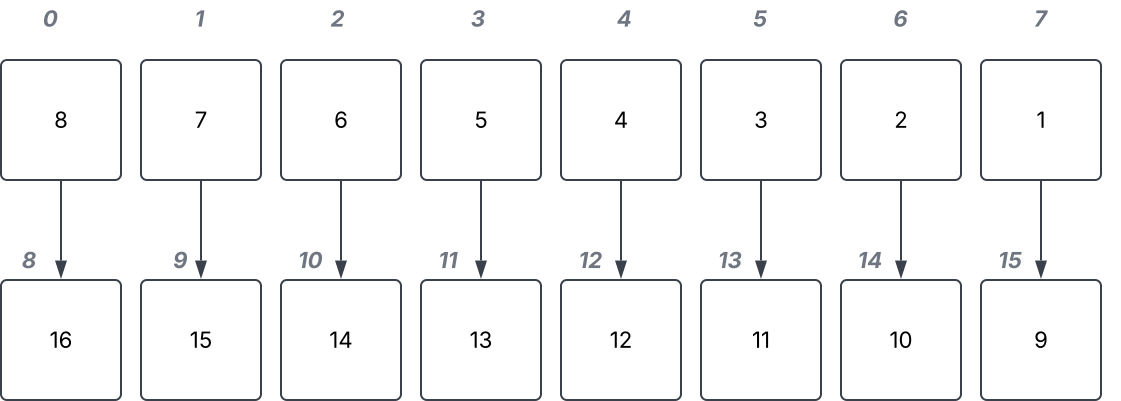
\includegraphics[width=1\columnwidth]{img/bestcase-it1}
    \caption{After the first pass, elements are relatively sorted within their respective $h_3$-spaced subsequences.}
    \label{fig:bestcase-it1}
\end{figure}

Subsequent passes continue processing the array and produce relatively sorted subsequences at decreasing distances: $h_2 = 4$ (Fig.~\ref{fig:bestcase-it2}), $h_1 = 2$ (Fig.~\ref{fig:bestcase-it3}), and finally $h_0 = 1$ (Fig.~\ref{fig:bestcase-it4}).

\begin{figure}[!h]
    \centering
    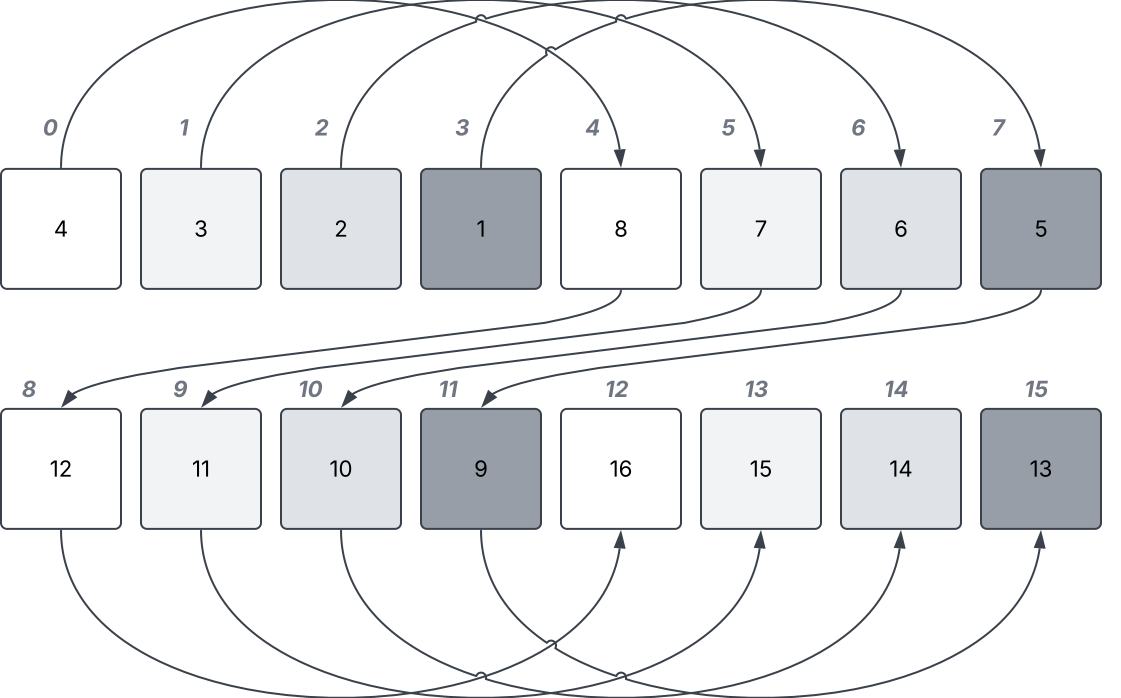
\includegraphics[width=1\columnwidth]{img/bestcase-it2}
    \caption{After the second pass, elements are relatively sorted at a gap of $h_2=4$.}
    \label{fig:bestcase-it2}
\end{figure}

\begin{figure}[!h]
    \centering
    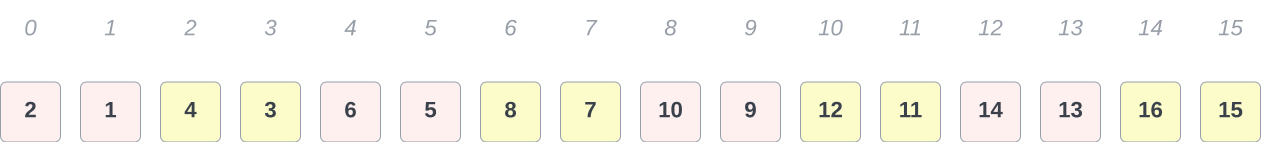
\includegraphics[width=1\columnwidth]{img/bestcase-it3}
    \caption{The third pass processes $h_1 = 2$-spaced elements, further refining local order.}
    \label{fig:bestcase-it3}
\end{figure}

\begin{figure}[!h]
    \centering
    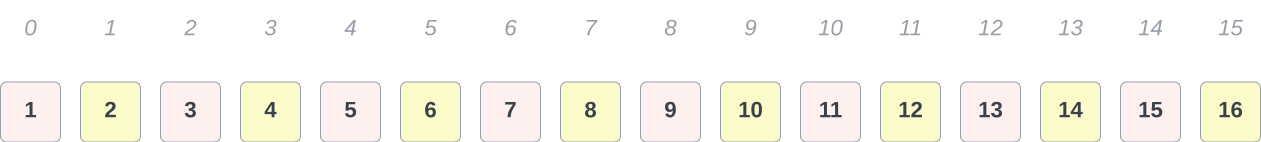
\includegraphics[width=1\columnwidth]{img/bestcase-it4}
    \caption{The final pass performs an insertion-sort-like operation with $h_0 = 1$, yielding the fully sorted array.}
    \label{fig:bestcase-it4}
\end{figure}

To estimate $c_3$, we consider the number of element comparisons performed in the innermost \texttt{while}-loop, where the algorithm checks whether elements at positions $j$ and $j - \texttt{delta}$ need to be reordered.
For our strictly descending input array of size $n = 2^4$, this condition is always satisfied during each comparison, leading to the maximum number of element swaps per pass.
Since there are $\frac{n}{2}$ such comparisons per pass, the total number of $c_3$ calls can be approximated by:

\[
    \lg n\ \cdot \frac{n}{2}
\]
\noindent
Additionally, including the contributions from $c_1$ and $c_2$ as derived earlier

\[
    c_1 = \lg n, \quad
    c_2 = n \cdot \lg(n) - n + 1
\]

\noindent
the total number of steps is a combination of comparisons, iterations and passes, and sums up to:

\[
    \lg(n) + n \cdot \lg(n) - n + 1 + \lg(n) \cdot \frac{n}{2}
\]

\noindent
For our specific case with $n = 16$, this yields
\[
    \lg(16) + 16 \cdot \lg(16) - 16 + 1 +  \lg(16) \cdot \frac{16}{2} = 85
\]

\begin{theorem}[Asymptotic Bound for strictly ordered arrays]
    For arrays that are initially sorted in strictly descending order, Shellsort performs at most $O(n\ \lg\ n)$ sorting operations.
\end{theorem}

\begin{proof}
    We eliminate constant and lower-order terms from
    \[
        f(n) = \frac{3}{2} \cdot n\ \cdot \lg(n) + \lg(n) - n + 1
    \]
    \noindent
    leaving the dominant term in terms of growth with respect to $n$, which  is $lg(n) \cdot n$.
    To show that $f(n) \in O(n\ log\ n)$, we aim to find constants $c >0$ and $n_0 \in \mathbb{N}$ such that\footnote{
    see~\cite[11]{GD18a}
    }

    \[
       \forall n \geq n_0: f(n) \leq c \cdot n\ \cdot \lg\ n
    \]

    \noindent
    We prove the inequality
    \[
        \frac{3}{2} \cdot n \cdot \lg(n) + \lg(n) - n + 1 \leq c \cdot n \cdot \lg(n)
    \]

    \noindent
    Substituting $n_0 = 1$ and $c = \frac{3}{2}$, we observe that

    \[
        \forall n \geq n_0: \frac{3}{2} \cdot n \cdot \lg(n)  \leq \frac{3}{2} \cdot n \cdot \lg(n)
    \]

    \noindent
    holds trivially.
    Moreover, since $lg(n) < n$ for all $n \in \mathbb{N}$, it follows that $\lg(n) - n < 0$ and therefore $lg(n) - n + 1 \leq 0$.
    Hence, the entire expression satisfies
    \[
        f(n) \leq \frac{3}{2} \cdot n \cdot \lg(n)
    \]
    \noindent
    for all $n \geq 1$, and therefore $f(n) \in  O(n\ \lg\ n)$.
\end{proof}

